\chapter{Related Work}

In the following sections, we introduce four benchmark frameworks that are designed to investigate the performance of RDF databases. In the end of the chapter, we summarize the frameworks and also describe the main concepts in our work that introduces a new approach to the existing benchmark frameworks.

\section{Berlin SPARQL Benchmark}

The Berlin SPARQL Benchmark (BSBM) is settled in an e-commerce use case in which a set of products is offered by different vendors and consumers who posted reviews about the products~\cite{berlin}. BSBM measures the SPARQL query performance of RDF-based tools via realistic workloads of use case motivated queries. The benchmark defines three different use cases and a suite of benchmark queries---a \textit{mix} of queries---in each of them~\cite{berlin_specification}, simulating the search and navigation pattern of a consumer looking for a product. The queries include read and update operations as well.

BSBM generates artificial models in different sizes, by using normal distributions among the elements. For example, the number of reviews and different properties per products are distributed following a normal distribution.

The benchmark defines particular performance metrics that relate to the query execution times from different perspectives. The most important metrics are the following:
\begin{itemize}
	\item{\textit{Queries per Second}}: It is equal to the number of queries executed within a second.
	\item{\textit{Query Mixes per Hour}}: Denotes the number of mixed queries with different parameters that evaluated within an hour.
	\item{\textit{Overall Runtime}}: The overall time that a certain amount of query mix require.
\end{itemize}


\section{DBpedia SPARQL Benchmark}
The DBpedia SPARQL Benchmark (DBPSB) proposes a benchmark framework for RDF databases based on the DBpedia~\cite{dbpedia_data} knowledge base, and it measures the performance of real queries that were issued against existing RDF data~\cite{dbpedia}. DBPSB generates models in various sizes trying to obtain a similar characteristic belonging to the original DBpedia dataset.\\
Similarly to BSBM, DBPSB also defines metrics to investigate the performance from different aspects, such as the \textit{Query Mixes per Hour} and \textit{Queries per Second}. 

\section{SP$^2$Bench}

The SPARQL Performance Benchmark (SP$^2$Bench)~\cite{sp2bench} is based on the \textit{Digital Bibliography and Library Project} (commonly known as \textit{dblp}) which provides an open bibliographic information on major computer science publications~\cite{dblp}. The benchmark queries are not explicitly evaluated over the \textit{dblp} dataset, since SP$^2$Bench uses arbitrarily large, artificially generated models for the measurements that are created to follow the characteristics of the original \textit{dblp} dataset, such as the power-law distribution.

SP$^2$Bench is designed to test the most common SPARQL constructs, operator constellations and a broad range of RDF data access patterns. Instead of defining a sequence of use case motivated queries, the framework proposes various queries that cover specific RDF data management approaches.

Similarly to BSBM, SP$^2$Bench also measures additional performance related metrics besides the evaluation time, such as the disk storage cost, memory consumption, data loading time and success rates, hence, every metric captures different aspects from the evaluations.

\subsection{Train Benchmark Framework}\label{sec:train}

\begin{figure}[!ht]
	\centering
	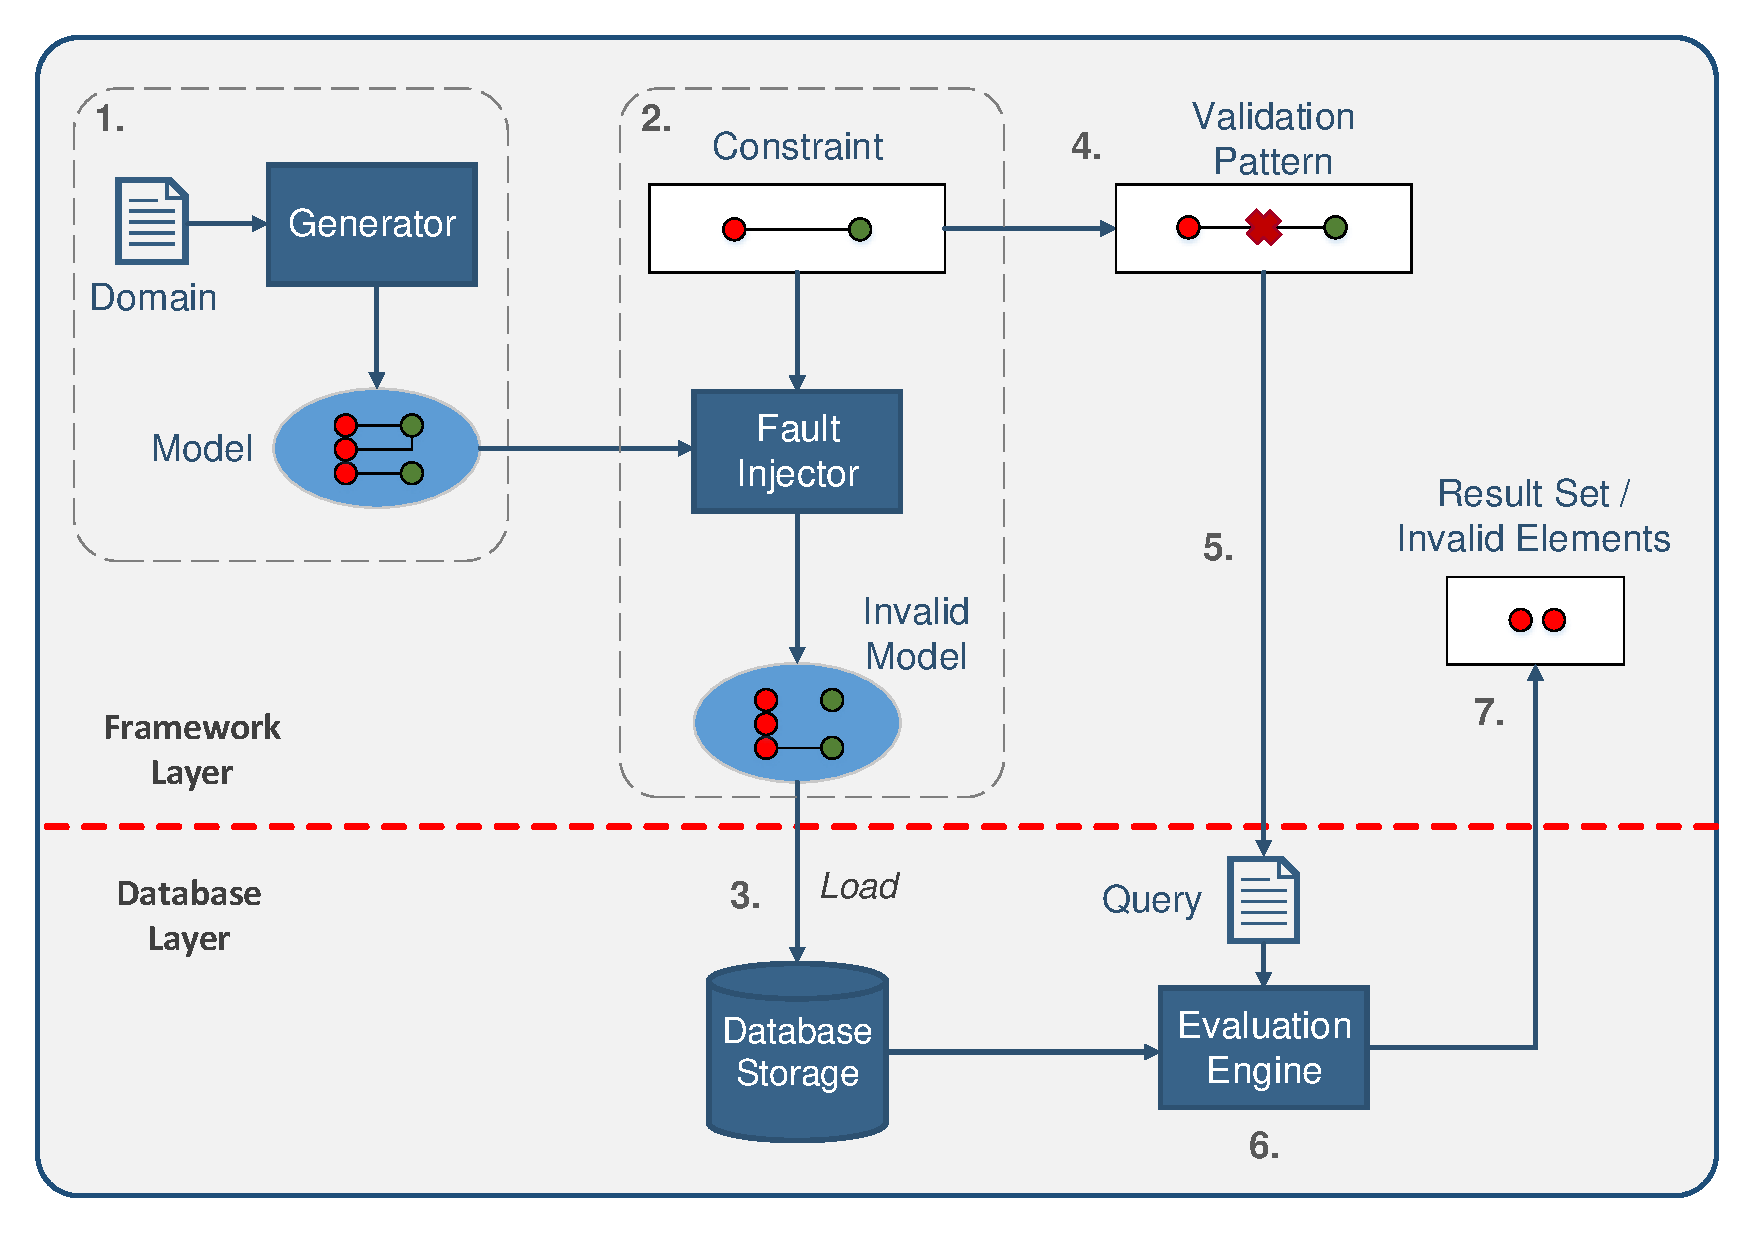
\includegraphics[width=150mm, keepaspectratio]{figures/functionality.pdf}
	\caption{An overview of Train Benchmark.}
	\label{fig:functionality}
\end{figure}

Short overview: well-formedness constraints + model validations, transformations.\\
Extended scope: RDF, EMF, SQL, Graphml.
Domain disadvantages. Emphasize this as common problems.

What is not mentioned: workflow, components, tools, detailed generator


The original domain of the Train Benchmark framework (introduced in \ref{section:metamodel} is not applicable for our goals to analyze graph queries, and study model - performance relationships. The main problems connecting to the domain are summarized in the following list:
\begin{enumerate}
	\item The original domain is not related to a real-life model, which leads to the fact that the cardinalities of the elements and their relationships do not follow a real model's characteristic, therefore, the measurement results of different tools cannot be claimed to be representative in a real-life use case. \label{item:railway_problem1}
	\item Besides the origin of the domain, the second problem is that the artificially generated models do not cover a well-known topology or degree distribution that can be observed in actual networks. \label{item:railway_problem2}
	\item Finally, the generated models of Train Benchmark are not capable of attaching arbitrary connections between the elements. \label{item:railway_problem3}
\end{enumerate}

Obviously, problem \ref{item:railway_problem2} is relevant to the generator component's insufficiency, since a representative distribution can be achieved independently on the domain, however, in order to generate arbitrary distributions, it is essential to guarantee a solution for problem \ref{item:railway_problem3}.

Problem \ref{item:railway_problem3} requires some explanation. In order to construct graphs with different degree distributions, it is an essential expectation of the domain to contain self-references, thus indicating that any of the vertices can be adjacent. In addition, the presence of a self-reference should be also interpretable conceptually in the domain. 

Considering the original domain, the type \textsf{Segment} represents the majority of the elements, however---without breaking the original meaning of the domain---we cannot make connection between any of the segments.


To summarize, a new domain is necessary that is related to a real-life model, and also suited to use for generating different distributions.


\subsection{Conclusions} \label{sec:benchmark_conclusions}

One common attribute of the previously introduced benchmark frameworks is that they lack precise analysis of searching connection between model characteristic and evaluation performance. In these frameworks, it is not supported to assess a tool's performance on different topologies, still using the same domain. Generally, the frameworks propose the generation of variously large models, thus investigating scalability, however, they do not focus on modifying the internal structures of the models, and generate different topologies, even in the same size.

model -> real
real life use cases
systematic queries
realistic workloads
model modifications
static model
scalability
metrics

%todo more? metrics? prob dist? use case?
